\documentclass[10pt]{extarticle}

\usepackage[utf8]{inputenc}
\usepackage[T1]{fontenc}
\usepackage{textcomp}

\usepackage{url}

% \usepackage{hyperref}
% \hypersetup{
%     colorlinks,
%     linkcolor={black},
%     citecolor={black},
%     urlcolor={blue!80!black}
% }

\usepackage{graphicx}
\usepackage{float}
\usepackage[usenames,dvipsnames]{xcolor}

% \usepackage{cmbright}

\usepackage{amsmath, amsfonts, mathtools, amsthm, amssymb}
\usepackage{mathrsfs}
\usepackage{cancel}

% horizontal rule
\newcommand\hr{
    \noindent\rule[0.5ex]{\linewidth}{0.5pt}
}

\usepackage{tikz}
\usepackage{tikz-cd}

% theorems
\usepackage{thmtools}
\usepackage[framemethod=TikZ]{mdframed}
\mdfsetup{skipabove=1em,skipbelow=0em, innertopmargin=5pt, innerbottommargin=6pt}

\theoremstyle{definition}

\makeatletter

\declaretheoremstyle[headfont=\bfseries\sffamily, bodyfont=\normalfont, mdframed={ nobreak } ]{thmgreenbox}
\declaretheoremstyle[headfont=\bfseries\sffamily, bodyfont=\normalfont, mdframed={ nobreak } ]{thmredbox}
\declaretheoremstyle[headfont=\bfseries\sffamily, bodyfont=\normalfont]{thmbluebox}
\declaretheoremstyle[headfont=\bfseries\sffamily, bodyfont=\normalfont]{thmblueline}
\declaretheoremstyle[headfont=\bfseries\sffamily, bodyfont=\normalfont, numbered=no, mdframed={ rightline=false, topline=false, bottomline=false, }, qed=\qedsymbol ]{thmproofbox}
\declaretheoremstyle[headfont=\bfseries\sffamily, bodyfont=\normalfont, numbered=no, mdframed={ nobreak, rightline=false, topline=false, bottomline=false } ]{thmexplanationbox}


\declaretheorem[numberwithin=chapter, style=thmgreenbox, name=Definition]{definition}
\declaretheorem[sibling=definition, style=thmredbox, name=Corollary]{corollary}
\declaretheorem[sibling=definition, style=thmredbox, name=Proposition]{prop}
\declaretheorem[sibling=definition, style=thmredbox, name=Theorem]{theorem}
\declaretheorem[sibling=definition, style=thmredbox, name=Lemma]{lemma}



\declaretheorem[numbered=no, style=thmexplanationbox, name=Proof]{explanation}
\declaretheorem[numbered=no, style=thmproofbox, name=Proof]{replacementproof}
\declaretheorem[style=thmbluebox,  numbered=no, name=Exercise]{ex}
\declaretheorem[style=thmbluebox,  numbered=no, name=Example]{eg}
\declaretheorem[style=thmblueline, numbered=no, name=Remark]{remark}
\declaretheorem[style=thmblueline, numbered=no, name=Note]{note}

\renewenvironment{proof}[1][\proofname]{\begin{replacementproof}}{\end{replacementproof}}

\AtEndEnvironment{eg}{\null\hfill$\diamond$}%

\newtheorem*{uovt}{UOVT}
\newtheorem*{notation}{Notation}
\newtheorem*{previouslyseen}{As previously seen}
\newtheorem*{problem}{Problem}
\newtheorem*{observe}{Observe}
\newtheorem*{property}{Property}
\newtheorem*{intuition}{Intuition}


\usepackage{etoolbox}
\AtEndEnvironment{vb}{\null\hfill$\diamond$}%
\AtEndEnvironment{intermezzo}{\null\hfill$\diamond$}%




% http://tex.stackexchange.com/questions/22119/how-can-i-change-the-spacing-before-theorems-with-amsthm
% \def\thm@space@setup{%
%   \thm@preskip=\parskip \thm@postskip=0pt
% }

\usepackage{xifthen}

\def\testdateparts#1{\dateparts#1\relax}
\def\dateparts#1 #2 #3 #4 #5\relax{
    \marginpar{\small\textsf{\mbox{#1 #2 #3 #5}}}
}

\def\@lesson{}%
\newcommand{\lesson}[3]{
    \ifthenelse{\isempty{#3}}{%
        \def\@lesson{Lecture #1}%
    }{%
        \def\@lesson{Lecture #1: #3}%
    }%
    \subsection*{\@lesson}
    \testdateparts{#2}
}

% fancy headers
\usepackage{fancyhdr}
\pagestyle{fancy}

% \fancyhead[LE,RO]{Gilles Castel}
\fancyhead[RO,LE]{\@lesson}
\fancyhead[RE,LO]{}
\fancyfoot[LE,RO]{\thepage}
\fancyfoot[C]{\leftmark}
\renewcommand{\headrulewidth}{0pt}

\makeatother

% figure support (https://castel.dev/post/lecture-notes-2)
\usepackage{import}
\usepackage{xifthen}
\pdfminorversion=7
\usepackage{pdfpages}
\usepackage{transparent}
\newcommand{\incfig}[1]{%
    \def\svgwidth{\columnwidth}
    \import{./figures/}{#1.pdf_tex}
}

% %http://tex.stackexchange.com/questions/76273/multiple-pdfs-with-page-group-included-in-a-single-page-warning
\pdfsuppresswarningpagegroup=1

\author{Gilles Castel}

\makeindex

\title{Tutorium MfP4 - SoSe 25}
\author{zur Vorlesung von PD Dr. Holtkamp}
\date{\today} % Replace with \today to show the current date

\begin{document}
\let\temp\phi
\let\phi\varphi
\let\varphi\temp
\maketitle

\definecolor{tcol_CNT1}{HTML}{72E094} % First color for Contents
\definecolor{tcol_CNT2}{HTML}{24E2D6} % Second color for Contents
\definecolor{tcol_CNV1}{HTML}{8E44AD} % First color for Conventions
\definecolor{tcol_CNV2}{HTML}{A10B49} % First color for Conventions

\begin{tcolorbox}[enhanced,
    title=Inhaltsverzeichnis,
    fonttitle=\fontsize{20}{24}\sffamily\bfseries\selectfont,
    coltitle=black,
    fontupper=\sffamily,
    attach boxed title to top center={yshift=10pt},
    boxed title style={frame hidden,
        interior style={left color=tcol_CNT1!0,right color=tcol_CNT2!0},
        frame style={left color=tcol_CNT1!0!black,right color=tcol_CNT2!0!black},
        height=24pt,bean arc,drop fuzzy shadow
    },
    top=2mm,bottom=2mm,left=2mm,right=2mm,
    before skip=20mm,after skip=20mm,
    drop fuzzy shadow,breakable]
%
\makeatletter
\@starttoc{toc}
\makeatother
\end{tcolorbox}

\begin{tcolorbox}[enhanced,
    title=Konventionen,
    fonttitle=\large\sffamily\bfseries\selectfont,
    boxrule=2pt,left=2pt,right=2pt,
    attach boxed title to top left,
    top=2mm,bottom=2mm,left=2mm,right=2mm,
    before skip=10mm,after skip=10mm]
%
\begin{itemize}
\item Wir schreiben für einen Körper $\K$ kurz $\K^\ast := \K \exc \{0\}$.
\item Real- und Imaginärteil werden mit $\Re(\cdot)$ respektive $\Im(\cdot)$ bezeichnet, das Bild einer Abbildung $f$ hingegen mit $\im (f)$.
\item Echte Teilmengen tragen das Symbol $\subset$, allgemeine Teilmengen das Symbol $\sub$.
\end{itemize}
\end{tcolorbox}
Dies sind meine Tutoriumsnotizen für Mathe für Physiker 4. Falls Ihr Fehler findet, sagt immer gerne Bescheid. Allgemein sind die Notizen oft schnell von mir für meine eigene Tutoriumsvorbereitung getippt, erwartet also bitte kein voll ausgearbeitetes \LaTeX-Skript.
\newpage 
\sloppy
\section{Tutorium 10.04.25}
\label{sec:10_04_25}

\subsection{Organisatorisches}
\begin{itemize}
\item Festlegung des allgemeinen Tutoriumtermins. Ort: Voraussichtlich wieder Geomatikum, wenn Raum verfügbar.
\item Fahrplan MfP4: Differentialgeometrie, Funktionentheorie, Funktionalanalysis
\item Wünsche für das Tutorium? Vergleich letzte Semester, konkrete Vorstellungen, etc.
\item MathNet-Wolke, Moodle, Homepage, Telegram-Gruppe
\end{itemize}

\subsection{Literaturempfehlungen}
Zur Differentialgeometrie kennt ihr bereits meine Empfehlungen von letztem Semester.
Zur Funktionentheorie:
\begin{itemize}
\item Jänich, \href{https://link.springer.com/book/10.1007/3-540-35015-2}{Funktionentheorie}: Sehr angenehm zu lesendes Buch, vor allem, wenn man vielleicht auch an gut geschriebenen Büchern und Anekdoten Spaß hat. 
\item Salamon, \href{https://link.springer.com/book/10.1007/978-3-0348-0169-0}{Funktionentheorie}: Das Buch basiert auf Ahlfors, Complex Analysis, einem beachtlich guten Standardwerk im englischen Raum. Etwas trockener als Jänich, eher im typischen Mathe-Stil.
\item Needham, \href{https://umv.science.upjs.sk/hutnik/NeedhamVCA.pdf}{Visual Complex Analysis}: Das (englischsprachige) Buch kann man am besten nebenher lesen, wenn man sich für die geometrische Intuition hinter der Funktionentheorie interessiert.
\end{itemize}
Zur Funktionalanalysis:
Hier ist das Skript kaum zu schlagen, da die Themenwahl wirklich sehr speziell auf das Notwendigste für die Physik gelegt wurde. Die meisten Mathebücher würden die Konzepte aus dem zweiten Semesterteil auf zwei ganze Semester aufteilen. Und dazu kommt noch mehr Maßtheorie\dots. Nichtsdestotrotz, ein bisschen was fällt mir ein:
\begin{itemize}
\item Kaballo, \href{https://link.springer.com/book/10.1007/978-3-662-54748-9}{Grundkurs Funktionalanalysis}: Das Buch ist aus einem MfP-ähnlichen Modul entstanden und daher einigermaßen geeignet. Allgemein ist das Buch relativ nett geschrieben.
\item Hall, \href{https://link.springer.com/book/10.1007/978-1-4614-7116-5}{Quantum Theory for Mathematicians}: Hier wird die Funktionalanalysis aus Sicht der Physik mit mittelmäßigem mathematischen Anspruch betrachtet. Mathematisch streng veranlagte Leute können mit dem Buch oft nicht so viel anfangen, manchen gereicht es aber auch zur Rettung. Einfach mal reinlesen :)
\end{itemize}
Im Allgemeinen ist MfP4 meiner Erfahrung nach, vor allem wenn noch Differentialgeometrie abgefragt wird, sehr gut machbar, vor allem im Vergleich zu den sehr dichten MfP2- und MfP3-Modulen. Erfahrungsgemäß mögen viele die Funktionentheorie sehr und können damit gut umgehen. Funktionalanalysis fällt hingegen meist schwer, da das Thema vielen weniger intuitiv scheint. Im besten Fall findet man aber an beidem Gefallen, im schlimmsten Fall kommt man mit DiffGeo und Funktionentheorie sicher durch die Klausur.



\section{Tutorium 17.04.25}
\label{sec:17_04_25}

\subsection{Wiederholung - Komplexe Zahlen}
Mit Sicherheit erinnert ihr euch noch gut an die komplexen Zahlen:
\begin{definition}{Komplexe Zahlen}{komplexezahlen}
Der Körper $(\C, +, \cdot)$ mit
\begin{equation}
\C := \{(a,b) \in \R \mid a,b \in \R\}
\end{equation}
und den Operationen
\begin{equation}
\begin{split}
+: \C \times \C &\to \C\\
(a,b), (c,d) &\mapsto (a,b) + (c,d) := (a+c,b+d),
\end{split}
\end{equation}
genannt Addition, und
\begin{equation}
\begin{split}
\cdot: \C \times \C &\to \C\\
(a,b),(c,d) &\mapsto (a,b) \cdot (c,d) := (ac-bd, ad+bc),
\end{split}
\end{equation}
genannt Multiplikation, nennen wir den Körper der \textbf{komplexen Zahlen}. Die Zahl $a=\Re(a,b)$ heißt \textbf{Realteil}, die Zahl $b=\Im(a,b)$ \textbf{Imaginärteil} von $z$. 
\end{definition}
Meist führt man die \textit{komplexe Einheit} $i$ ein, sodass $(a,b)=a+bi$ für $i^2:=-1$ gilt. Dies erleichtert Rechnungen, ist aber rein symbolischer Natur. Fundamental ist, dass hier ein Körper vorliegt: Sowohl $(\C, +)$ als auch $(\C^\ast, \cdot)$ sind Gruppen (das könnt ihr gerne zur Übung nachprüfen, vor allem die Inversen sollte man einmal konstruiert haben). Bereits aus MfP1 kennt ihr die \textit{komplexe Konjugation}
\begin{equation}
\begin{split}
\overline{\cdot}: \C &\to \C\\
z = a+bi &\mapsto \overline{z} := a-bi.
\end{split}
\end{equation}
Geometrisch entspricht dies einer Spiegelung an der reellen Achse. Auf $\C$ definieren wir außerdem den \textit{Absolutwert} oder \textit{Betrag} durch
\begin{equation}
\begin{split}
|\cdot |: \C &\to \C\\
z &\mapsto |z| := \sqrt{z \overline{z}} = \sqrt{\Re(z)^2+\Im(z)^2}
\end{split}
\end{equation}
mit einigen wichtigen Eigenschaften:
\begin{enumerate}[({M}1)]
\item Positivität: $|z| \geq 0$ mit $|z| = 0 \iff z=0$
\item Multiplikativität: $|z_1z_2| = |z_1||z_2|$
\item Subadditivität (Dreiecksungleichung): $|z_1+z_2| \leq |z_1| + |z_2|$.
\end{enumerate}
Sowohl die Multiplikativität als auch die Subadditivität kann man induktiv auf beliebige \red{endliche} Produkte bzw. Summen ausweiten.\\
Damit erhalten wir eine Möglichkeit, aus geometrischen Überlegungen verschiedene Formen für komplexe Zahlen herzuleiten. Ausgehend von der \textit{kartesischen Form} $z=a+bi$ definieren wir den \textbf{Radius} von $z$ als $r := |z|$. Das \textbf{(Haupt-)Argument} von $z$ ist dessen eingeschränkter Polarwinkel $\phi \in (-\pi, \pi]$, das aus trigonometrischen Überlegungen hergeleitet werden kann. Damit erhalten wir die \textit{Polarform} und mit der Eulerschen Formel auch die \textit{trigonometrische Form}:
\begin{equation}
z = r \exp(i\phi) = r(\cos \phi + i \sin \phi).
\end{equation} 
\begin{figure}[H]
\centering
\begin{tikzpicture}[scale=3]
	\draw[step=.5cm, gray, very thin, dotted] (-1.4,-1.4) grid (1.4,1.4);
	\foreach \x/\xtext in {-1, 1}
		\draw (\x,-1pt) -- (\x, 1pt) node[anchor=north] {$\xtext$};
	\foreach \y/\ytext in {-1, 1}
		\draw (-1pt, \y) -- (1pt, \y) node[anchor=east, left=2pt] {$\ytext$};
	\draw[->] (-1.5,0) -- (1.5,0);
	\draw[->] (0,-1.5) -- (0,1.5);
	\draw (0,0) circle [radius=1cm];
	\draw (.5cm,0) arc [start angle=0, end angle=40, radius=.5cm] node[right=1pt,pos=0.5] {$\phi$};
	\draw[red] (40:1cm) -- node[right=1pt, thick] {$\sin \phi = \Im(z)$} (40:1cm |- 0,0);
	\draw[blue] (0,0) -- node[below=4pt,pos=0.5, thick] {$\cos \phi = \Re(z)$} (40:1cm |- 0,0);
	\draw (0,0) -- node[above=2pt, thick] {$r$}  (40:1cm) node[black, right=1pt] {$z$};
	\filldraw[black] (40:1cm) circle [radius=0.5pt];
\end{tikzpicture}
\caption{Die Einheitskreislinie $\S^1 \hookrightarrow \C$ mit der komplexen Zahl $z=r\exp(i\phi)$.}
\end{figure}
Nicht immer ist es ganz so einfach, das Argument aus der kartesischen Form zu ermitteln. Wir illustrieren dies mal wie folgt:
\begin{figure}[H]
\centering
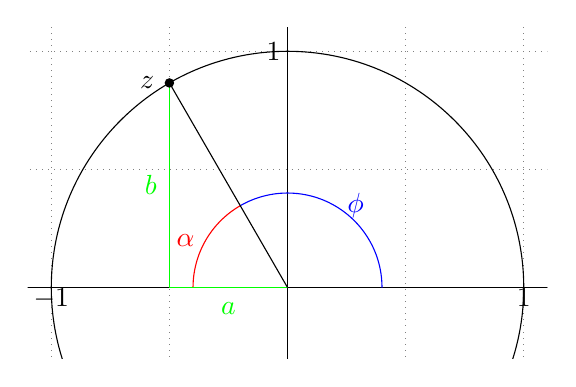
\begin{tikzpicture}[scale=3]
	\clip (-1.1, -0.3) rectangle (1.1, 1.1);
	\draw[step=.5cm, gray, very thin, dotted] (-1.4,-1.4) grid (1.4,1.4);
	\foreach \x/\xtext in {-1, 1}
		\draw (\x,-1pt) -- (\x, 1pt) node[anchor=north] {$\xtext$};
	\foreach \y/\ytext in {-1, 1}
		\draw (-1pt, \y) -- (1pt, \y) node[anchor=east, left=2pt] {$\ytext$};
	\draw[->] (-1.5,0) -- (1.5,0);
	\draw[->] (0,-1.5) -- (0,1.5);
	\draw (0,0) circle [radius=1cm];
	\draw[blue] (.4cm,0) arc [start angle=0, end angle=120, radius=.4cm] node[right=1pt,pos=0.5] {$\phi$};
	\draw[red] (-.4cm,0) arc [start angle=180, end angle=120, radius=.4cm] node[left=.5pt, pos=0.5] {$\alpha$};
	\draw[green] (120:1cm) --  (120:1cm |- 0,0) node[left=1pt,pos=0.5] {$b$} ;
	\draw[green] (0,0) -- node[below=2pt] {$a$} (120:1cm |- 0,0) ;
	\draw (0,0) --   (120:1cm) node[black, left=2pt] {$z$};
	\filldraw[black] (120:1cm) circle [radius=0.5pt];
\end{tikzpicture}
\caption{In diesem Fall lässt sich der Polarwinkel von $z=a+ib$ nicht direkt ableiten. Wir erhalten $\cos \alpha = \frac{|a|}{\sqrt{a^2+b^2}}$ und damit $\phi = \pi - \arccos(\frac{|a|}{\sqrt{a^2+b^2}}) = \arccos(\frac{a}{\sqrt{a^2+b^2}})$. Dabei nutzt man, dass $\arccos(x) = \pi - \arccos(-x)$ gilt.}
\end{figure}
Wir wollen nun die wichtigen topologischen Begriffe auf $\C$ betrachten. Die Topologie der komplexen Ebene wird von der Metrik induziert:
\begin{definition}{Topologie auf $\C$}{epsilonball}
Der \textbf{offene $\epsilon$-Ball} in $\C$ ist die Teilmenge 
\begin{equation}
B_\epsilon(z) := \{x \in \C \mid |z-x| < \epsilon\}
\end{equation}
mit Radius $\epsilon$ und Mittelpunkt $z$. Eine Teilmenge $X \sub \C$ ist genau dann offen, wenn für alle $z \in X$ gilt, dass $B_\epsilon(z) \sub X$ für ein $\epsilon>0$ erfüllt ist.
\end{definition}
Man erinnere sich daran, dass eine abgeschlossene Menge darauf aufbauend definiert ist: Eine Teilmenge $A \sub \C$ heißt \textit{abgeschlossen}, wenn ihr Komplement $\C \setminus A$ offen ist. Eine Menge kann sowohl abgeschlossen als auch offen sein. Wir brauchen noch weitere Grundbegriffe der Topologie:
\begin{definition}{Zusammenhang und Gebiet}{gebiet}
\begin{enumerate}[(i)]
\item Eine Teilmenge $A \sub \C$ heißt \textbf{zusammenhängend}, wenn sie sich nicht in zwei \textcolor{red}{offene, disjunkte, nicht-leere} Teilmengen zerlegen lässt. Äquivalent dazu ist, dass bei einer Zerlegung $A = B \cup C$ mit $B,C$ offen und disjunkt $A$ oder $B$ die leere Menge sein muss.
\item Eine Teilmenge $A \sub \C$ heißt \textbf{Gebiet}, wenn sie zusammenhängend, offen und nicht-leer ist.
\end{enumerate}
\end{definition}

Mit diesem Wissen sollte es uns leichter fallen, Teilmengen von $\C$ zu charakterisieren. Das versuchen wir zur Übung gleich einmal:
\begin{übung}
Skizziere folgende Teilmengen von $\C$:
\begin{enumerate}[(a)]
\item $M_1 := \{z \in \C \mid 3 \leq |z| \leq 10 \}$
\item $M_2 := \{z \in \C \mid \Re(z^2) > 0 \}$
\item $M_3 := \{z \in \C^\ast \mid \Re \left( \frac{1}{z}\right) \leq 2\}$
\end{enumerate}
Entscheide außerdem, ob die angegebenen Mengen Gebiete (in der von der Metrik induzierten Topologie) sind.
\end{übung}
\begin{lösung}
\begin{enumerate}[(a)]
\item Hier hat man wahrscheinlich schon ein Bild vor Augen, denn wenn man die Polardarstellung $z=r\exp(i \phi)$ einsetzt, erhält man unmittelbar 
\begin{equation}
	3 \leq |r| \leq 10,
\end{equation}
da $|\exp(i \phi)|=1$. Wir erhalten also einen \textit{Kreisring}, wie unten abgebildet. Die Menge ist außerdem offensichtlich nicht offen, denn jeder Randpunkt $z \in \partial M_1$ besitzt keinen offenen $\epsilon$-Ball $B_\epsilon(z)$, der noch ganz in $M_1$ liegt. Also kann $M_1$ kein Gebiet sein.
\item Wir setzen $z=a+bi$ an und erhalten die Ungleichung 
\begin{equation}
\Re((a+bi)^2) = \Re(a^2-b^2+2iab)=a^2-b^2 >0.
\end{equation}
Dies ist äquivalent zu $a^2 > b^2$, die Menge wird also nach unten beschränkt durch die Raumdiagonalen $\Delta_{(a,a)}$ und $\Delta_{(a,-a)}$. Wir erhalten den Longitudinalschnitt eines Kegels, wobei der Ursprung ausgenommen wird. Diese Menge ist offen, denn für alle $z \in M_2$ liegt der offene $\epsilon$-Ball mit $\epsilon<\frac{a}{2}$ für beliebiges $a$ auf der Diagonale noch ganz in $M_2$. Jedoch ist die Menge kein Gebiet, da sie nicht zusammenhängend ist.
\item Wir setzen erneut $z=a+bi$ an und machen folgende Feststellung:
\begin{equation}
\frac{1}{z}=\frac{1}{a+bi}=\frac{a-bi}{(a+bi)(a-bi)}=\frac{a}{a^2+b^2} - i \frac{b}{a^2+b^2}.
\end{equation}
Also ist die Ungleichung durch 
\begin{equation}
\frac{a}{a^2+b^2} \leq 2 \iff 0 \leq a^2 - \frac{a}{2} +b^2
\end{equation}
gegeben. Quadratische Ergänzung liefert
\begin{equation}
0 \leq \left( a - \frac{1}{4} \right)^2 - \frac{1}{16} + b^2 \iff \left( \frac{1}{4} \right)^2 \leq \left( a - \frac{1}{4} \right)^2 +b^2,
\end{equation}
was gerade die Gleichung eines Kreises mit Radius $\frac{1}{4}$ darstellt, der auf $\left( \frac{1}{4},0\right)$ zentriert ist. Man sollte beachten, dass die Ungleichung so gestellt ist, dass die Menge ganz $\C$ ohne den Inhalt des Kreises darstellt. Dies ist aus den gleichen Gründen wie für $M_1$ kein Gebiet, denn die Punkte auf der Kreislinie haben keine offene Umgebung in $M_3$.
\end{enumerate}
\begin{figure}[H]
\centering
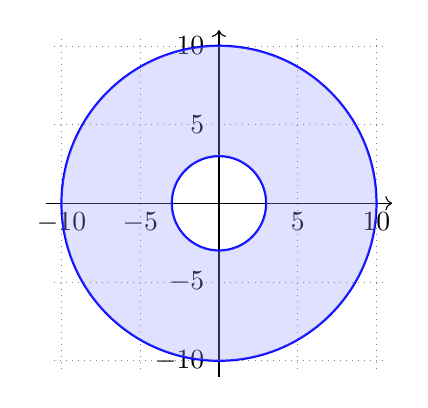
\begin{tikzpicture}[scale=.2]
	\draw[step=5cm, gray, very thin, dotted] (-10.5,-10.5) grid (10.5,10.5);
	\foreach \x/\xtext in {-10,-5,5,10}
		\draw (\x,-1pt) -- (\x, 1pt) node[anchor=north] {$\xtext$};
	\foreach \y/\ytext in {-10,-5,5,10}
		\draw (-1pt, \y) -- (1pt, \y) node[anchor=east, left=2pt] {$\ytext$};
	\draw[->] (-11,0) -- (11,0);
	\draw[->] (0,-11) -- (0,11);
	\draw[thick, blue] (0,0) circle [radius=3];
	\draw[thick, blue] (0,0) circle [radius=10];
	\fill[blue!40, opacity=.3, even odd rule] (0,0) circle [radius=3] (0,0) circle [radius=10];
\end{tikzpicture}
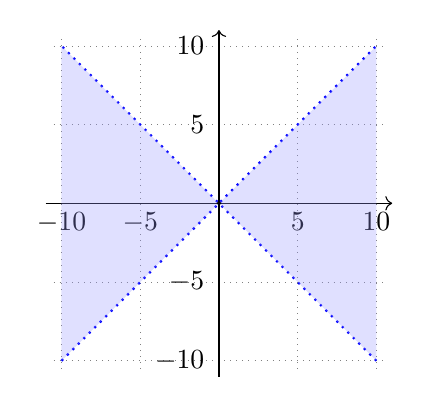
\begin{tikzpicture}[scale=.2]
	\draw[step=5cm, gray, very thin, dotted] (-10.5,-10.5) grid (10.5,10.5);
	\foreach \x/\xtext in {-10,-5,5,10}
		\draw (\x,-1pt) -- (\x, 1pt) node[anchor=north] {$\xtext$};
	\foreach \y/\ytext in {-10,-5,5,10}
		\draw (-1pt, \y) -- (1pt, \y) node[anchor=east, left=2pt] {$\ytext$};
	\draw[->] (-11,0) -- (11,0);
	\draw[->] (0,-11) -- (0,11);
	\draw[thick, blue, dotted] (-10,-10) -- (10,10);
	\draw[thick, blue, dotted] (10,-10) -- (-10,10);
	\fill[blue!40, opacity=.3] (0,0) -- (10,-10) -- (10,10) -- cycle;
	\fill[blue!40, opacity=.3] (0,0) -- (-10,-10) -- (-10,10) -- cycle;
	\filldraw[black] (0,0) circle (.1);
\end{tikzpicture}
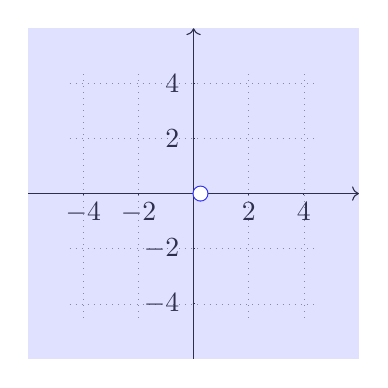
\begin{tikzpicture}[scale=.35]
	\draw[step=2cm, gray, very thin, dotted] (-4.5,-4.5) grid (4.5,4.5);
	\foreach \x/\xtext in {-4,-2,2,4}
		\draw (\x,-1pt) -- (\x, 1pt) node[anchor=north] {$\xtext$};
	\foreach \y/\ytext in {-4,-2,2,4}
		\draw (-1pt, \y) -- (1pt, \y) node[anchor=east, left=2pt] {$\ytext$};
	\draw[->] (-6,0) -- (6,0);
	\draw[->] (0,-6) -- (0,6);
	\draw[thick, blue] (0.25,0) circle [radius=0.25];
	\fill[blue!40, opacity=.3] (-6,-6) rectangle (6,6);
	\fill[white] (.25,0) circle (.25);
\end{tikzpicture}
\end{figure}
\end{lösung}
Eine weitere sehr wichtige Ungleichung wollen wir zur Übung beweisen:
\begin{satz}{Cauchy-Schwarz-Ungleichung}{cauchyschwarz}
Seien $x_1, \dots, x_n, y_1, \dots, y_n \in \C$ endlich viele komplexe Zahlen. Dann gilt die \textbf{Cauchy-Schwarz-Ungleichung}
\begin{equation}
\left| \sum_{i=1}^n x_i \overline{y}_i\right|^2 \leq \sum_{i=1}^n |x_i|^2 \sum_{i=1}^n |y_i|^2.
\end{equation}
\end{satz}
\begin{beweis}
Für den Beweis brauchen wir zwei Vorüberlegungen. Erst einmal bemerken wir, dass die Gleichung immer gilt, wenn $\sum_i |x_i|^2 \sum_i|y_i|^2 = 0$, da dann alle $x_i$ oder alle $y_i$ verschwinden müssen. Wir müssen den Beweis also nur noch für $\sum_i |x_i|^2 \sum_i|y_i|^2 > 0$ führen. Die andere Vorüberlegung ist etwas technisch\footnote{Wer denkt, die folgenden Umformungen fielen vom Himmel, kann versuchen, es von vorn nach hinten anzugehen. Dann ist es viel offensichtlicher.} Seien $\alpha, \beta, \gamma, \delta \in \R$. Da Quadrate reeller Zahlen immer positiv sind, stellen wir fest:
\begin{align*}
0 \leq (\alpha \delta- \beta \gamma)^2 &= \alpha^2\delta^2 + \beta^2 \gamma^2 -2\alpha \beta \gamma \delta\\
&= \blue{\alpha^2 \beta^2 - \alpha^2 \beta^2 + \gamma^2 \delta^2 - \gamma^2 \delta^2} +\alpha^2\delta^2 + \beta^2 \gamma^2 -2\alpha \beta \gamma \delta\\
&= (\alpha^2 + \gamma^2)(\beta^2+\delta^2) - (\alpha^2 \beta^2 + \gamma^2 \delta^2 + 2 \alpha \beta \gamma \delta)\\
&= (\alpha^2 + \gamma^2)(\beta^2+\delta^2) - (\alpha \beta + \gamma \delta)^2.
\end{align*}
Umstellen liefert nun eine Ungleichung, derer wir uns später bedienen:
\begin{equation}
(\ast)\, (\alpha \beta + \gamma \delta)^2 \leq (\alpha^2 + \gamma^2)(\beta^2+\delta^2).
\end{equation}
Nun beweisen wir endlich die Ungleichung mit vollständiger Induktion:\\
Für den Induktionsanfang brauchen wir nur (M2):
\begin{equation}
|x\overline{y}|^2 = (|x||\overline{y}|)^2 = |x|^2|y|^2.
\end{equation}
Hier gilt sogar Gleichheit. Die Induktionsvoraussetzung (IV) ist, dass die Aussage für $n-1$ gezeigt ist. Da beide Seiten positiv sind, können wir in der IV die Wurzel ziehen:
\begin{equation}
\left| \sum_{i=1}^{n-1} x_i \overline{y}_i\right| \leq \sqrt{\sum_{i=1}^{n-1} |x_i|^2} \sqrt{\sum_{i=1}^{n-1} |y_i|^2}.
\end{equation}
Für den Induktionsschritt müssen wir die Aussage für $n$ beweisen. Das geht nun relativ schnell:
\begin{align*}
\left| \sum_{i=1}^n x_i \overline{y}_i\right| &= \left| x_n \overline{y}_n + \sum_{i=1}^{n-1} x_i \overline{y}_i\right|\leq |x_n \overline{y}_n| + \left| \sum_{i=1}^{n-1} x_i \overline{y}_i\right|\\
&\leq^\text{\red{IV}} |x_n| |y_n| + \sqrt{\sum_{i=1}^{n-1} |x_i|^2} \sqrt{\sum_{i=1}^{n-1} |y_i|^2} \leq^{\red{(\ast)}} \sqrt{\sum_{i=1}^{n} |x_i|^2} \sqrt{\sum_{i=1}^{n} |y_i|^2}
\end{align*}
Im ersten Schritt haben wir die Dreiecksungleichung ausgenutzt, gefolgt von der Induktionsvoraussetzung. Den letzten Schritt können wir mit unserer Ungleichung $(\ast)$ direkt folgern, indem wir $\alpha:=|x_n|$, $\beta:= |y_n|$, $\gamma:= \sqrt{\sum_{i=1}^{n-1} |x_i|^2}$ und $\delta :=\sqrt{\sum_{i=1}^{n-1} |y_i|^2}$ setzen.
\end{beweis}
\section{Tutorium 24.04.25}
\label{sec:24_04_25}
Da sich das kommende Blatt ganz um Differentialformen drehen wird, wollen wir uns die neuen Begriffe zur Differentialgeometrie aus MfP4 nochmal genauer ansehen:
\subsection{Atlanten, Orientierungen und der Satz von Stokes}
Die zentrale Definition dieses Abschnittes ist die des Atlas:
\begin{definition}{Atlas}{atlas}
Sei $M$ eine $k$-Untermannigfaltigkeit des $\R^n$. Wir nennen eine Familie
\begin{equation}
\Af := \{\phi_j: T_j \to V_j\}_{j \in J}
\end{equation}
von \textit{lokalen Parametrisierungen} mit $\cup_{j \in J} V_j =M$ einen \textbf{Atlas} von $M$
\end{definition}
Was ist die Motivation hinter dieser Definiton? Um integrieren zu können, müssen wir das Verhalten einer Funktion $f:M \to \R^n$ charakterisieren können. Das Leitmotiv der Differentialgeometrie ist es, dafür die lokale Ähnlichkeit einer MFK auszunutzen: Ist $\psi: U \to \widehat{U}$ eine Karte mit $U \subset M$ und $\widehat{U} \sub \R^k$ offen, so können wir die Stetigkeit von $f$ auf die Stetigkeit von $f \circ \phi^{-1}: \R^k \to \R^n$ mit unseren gewohnten Definitionen zurückführen. Wir bemerken aber ein Problem: Atlanten sind nicht eindeutig. Wir wollen natürlich nicht, dass unsere Definition von der Wahl eines Atlas abhängt. 
Das Problem kann man auf mehrere Arten lösen, in der Vorlesung wurde das zusammen mit der Orientierung verpackt:
\begin{definition}{Orientierung}{orientierung}
Sei $M$ eine $k$-Untermannigfaltigkeit des $\R^n$. Existiert ein Atlas $\Af$ von $M$, sodass die Kartenwechselabbildung für sich schneidende Parametrisierungen orientierungserhaltend ist, heißt $M$ \textbf{orientierbar}. Können wir weitere lokale Parametrisierungen zu $\Af$ hinzufügen, ohne eine Änderung der Orientierung zu bewirken, heißen diese \textbf{positiv orientiert}, andernfalls \textbf{negativ orientiert}.\\
Wir fassen die Orientierung einer MFK als Äquivalenzklasse auf und bezeichnen $(M,\Af)$ als \textbf{orientierte MFK}.
\end{definition}
Das war eine ganz schöne Menge, aber jetzt haben wir, was wir wollten: Eine MFK ist entweder nicht orientierbar, oder es gibt genau zwei Orientierungen bzw. Äquivalenzklassen von Atlanten auf $M$. Im Skript wird fortan die positive Orientierung gewählt. Sind die lokalen Parametrisierungen von Klasse $\cC^\infty$, nennt man $\Af$ auch glatte Struktur auf $M$.\footnote{Wer diese Definition über Äquivalenzklassen nicht so hilfreich findet, kann auch mit \textbf{maximalen Atlanten} arbeiten: Ein Atlas $\Af$ heißt \textbf{maximal}, wenn er nicht die echte Teilmenge irgendeines anderen Atlas ist.}\\
Wir wollen nun Orientierungen auf $n-1$-dimensionale Hyperflächen ausweiten.
\begin{definition}{Orientierung des Tangentialraums}{orienttang}
Sei $(M, \Af)$ eine orientierte $k$-UMF des $\R^n$ mit positiv orientierter lokaler Parametrisierung $\phi$. Für jedes $p \in M$ ist 
\begin{equation}
(\partial_1 \phi_p, \dots, \partial_k \phi_p)
\end{equation}
eine positiv orientierte Basis von $T_pM$. Die Orientierung aller weiteren Basen wird relativ dazu festgesetzt.
\end{definition}
Für eine Hyperfläche $M \sub \R^{n\geq 2}$ mit Standardorientierung erhalten wir so ein bezüglich $\Af$ positiv orientiertes \textbf{Einheitsnormalenfeld} auf $M$: Dies ist ein stetiges Vektorfeld $\nu: M \to \R^n$, sodass für alle $p \in M$ $\nu(p)$ ein Einheitsnormalenvektor von $M$ ist und gilt: Ist $(v_1, \dots, v_{n-1})$ eine positiv orientierte Basis von $T_pM$, so ist $(\nu(p), v_1, \dots, v_{n-1})$ eine positiv orientierte Basis des $\R^n$. Die wahre Erkenntnis ist dabei:
\begin{satz}{Orientierung durch Einheitsnormalenfelder}{orientierungvektor}
Sei $M \sub \R^n$ eine Hyperfläche. Ist $M$ orientiert, so existiert ein positiv orientiertes Einheitsnormalenfeld. Existiert umkehrt ein Einheitsnormalenfeld auf $M$, so definiert dieses eine Orientierung der Hyperfläche.
\end{satz}
Das hilft uns schon einmal in der Vorstellung, wenn man bedenkt, dass Einheitsnormalenfelder für $2$-Mannigfaltigkeiten recht anschaulich sind. Darüber hinaus lässt sich so auch der Rand $\partial M$ einer MFK $M$ orientieren, indem man randadaptierte Parametrisierungen mit einheitlicher Orientierung auf den Rand einschränkt.
\begin{beispiel}
Betrachte das Möbiusband $M \sub \R^3$ und die $2$-Sphäre $\S^2 \sub \R^3$. Beide sind $2$-Mannigfaltigkeiten des $\R^3$. Man betrachte folgendes Bild:\\
\begin{center}
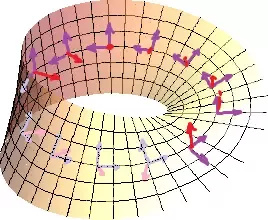
\includegraphics[scale=.3]{figures/mobius.png} 
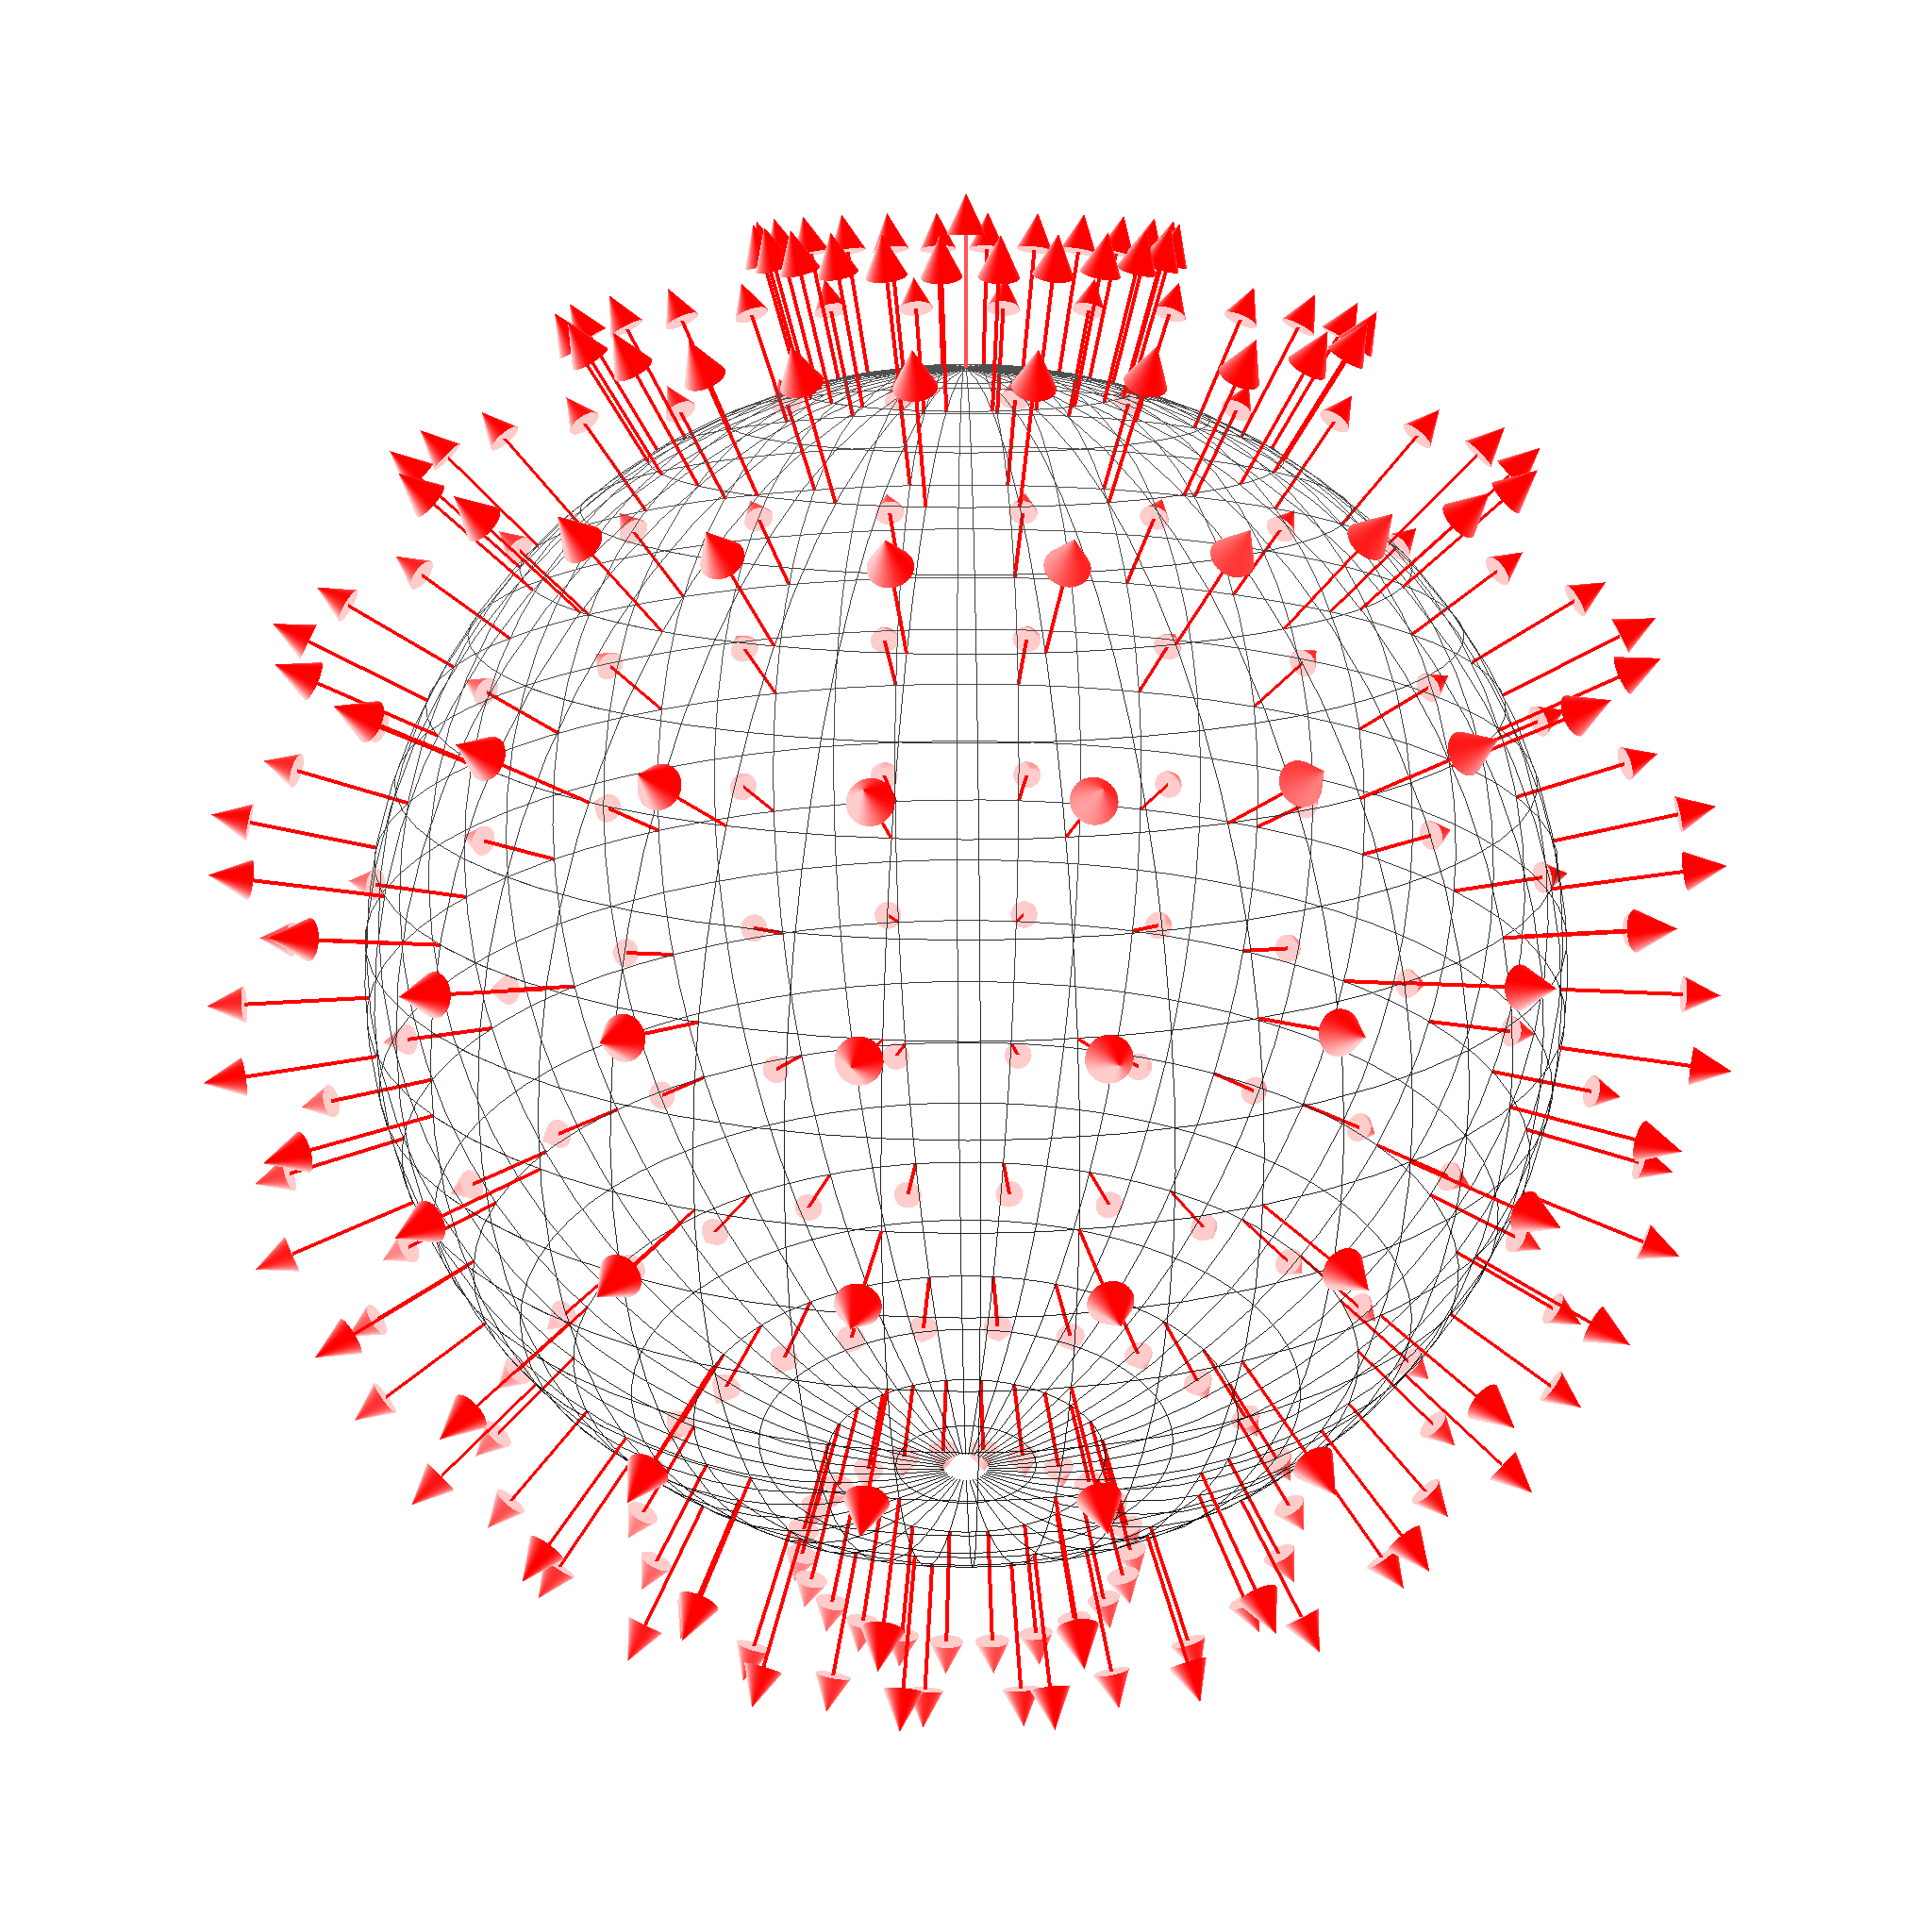
\includegraphics[scale=.05]{figures/sphere.png}
\end{center}
Erkennbar ist, dass sich das Möbiusband nicht orientieren lässt, während die Sphäre durch das Vektorfeld mit $\|v\|=1$ bereits positiv orientiert ist.
\end{beispiel}
Wir haben also jetzt alle Werkzeuge, um Integration auf der gesamten (Unter-)Mannigfaltigkeit über lokale Parametrisierungen zu verstehen. Ziel ist, eine stetige $k$-Form auf $U \sub \R^n$ über eine Teilmenge $A \sub M$ einer orientierten $k$-Untermannigfaltigkeit zu integrieren. Gibt es eine einzelne Parametrisierung $\phi: T \to V \sub M$ mit $A \sub V$, so definieren wir Integration über $A$ durch
\begin{equation}
\int_{(A, \Af)} \omega := \int_{\phi^{-1}(A)} \phi^\ast \omega.
\end{equation}
Andernfalls sei
\begin{equation}
\left( \phi_j: T_j \to V_j \sub M \right)_{j \in J}
\end{equation}
eine endliche Familie von lokalen Parametrisierungen mit $A \sub \cup_{j \in J} V_j$. Wir nehmen uns eine der Überdeckung $(V_j)_j$ untergeordnete Partition der Eins
\begin{equation}
\alpha_j: \bigcup_{l \in J} V_l \to \R
\end{equation}
her und teilen $A$ gewissermaßen auf die Träger der Partition der Eins auf mit $A_j := A \cap \supp(\alpha_j) \sub V_j$ . Jetzt können wir endlich integrieren: $\omega$ heißt \textit{integrierbar über} $A$, falls $\omega$ über alle $A_j$ integrierbar ist. Dann setzen wir
\begin{equation}
\int_{(A, \Af)} \omega := \sum_{j=1}^m \int_{\phi_j^{-1}(A_j)} (\alpha_j \circ \phi_j) \cdot (\phi_j^\ast \omega),
\end{equation}
zerstückeln das Integral also über die Partitionsmengen. Mit diesem Verständnis springen wir dann auch direkt zu einem der schönsten Sätze:
\begin{theorem}{Stokesscher Integralsatz}{stokes}
Sei $U \sub \R^n$ offen und $\omega$ eine glatte $(k-1)$-Form auf $U$ mit $k \geq 2$. Sei $M \sub U$ eine $k$-Untermannigfaltigkeit. Für jedes Kompaktum $A \sub M$ mit glattem Rand $\partial A$, orientiert durch $M$, gilt:
\begin{equation}
\int_A d\omega = \int_{\partial A} \omega.
\end{equation}
\end{theorem}
Daraus erhalten wir eine schöne Aussage für unberandete, kompakte Mannigfaltigkeiten $M$. Ist $M \sub U$ wie oben, aber $\partial M = \emptyset$, so erhalten wir direkt
\begin{equation}
\int_M d\omega = \int_\emptyset \omega = 0.
\end{equation}
Es gibt noch viele weitere schöne Aussagen, die daraus folgen und einen expliziten Zusammenhang zu exakten Differentialformen aufzeigen. Tatsächlich bekommen wir dadurch konkrete Äquivalenzen, die Exaktheit und Geschlossenheit mit bestimmten Integralen gleichsetzen. Für die Interessierten: Dies findet man unter den Stichworten \textit{De Rahm-Kohomologie} und \textit{De Rahm-Theorem}.
\section{Tutorium 08.05.25}
\label{sec:08_04_25}

Nachdem ihr nun voll in die Funktionentheorie eingestiegen seid, wollen wir uns damit etwas näher beschäftigen:
 
\subsection{Funktionentheorie ist \textit{nicht} reelle Analysis in zwei Variablen}
Wenn wir nun zur Analysis auf $\C$ übergehen, ist man leicht verleitet, den $\R-$\red{Vektorraum}-Isomorphismus $\C \cong \R^2$ so zu interpretieren, dass Funktionentheorie doch eigentlich nichts anderes sei als Analysis im $\R^2$. Das ist aber ein fataler Fehler! Der Schlüssel liegt darin, dass auf $\C$ eine andere Struktur, die Multiplikation mit komplexen Zahlen, definiert ist, die über die Vektorraumstruktur des $\R^2$ hinausgeht.\\
In der reellen Analysis war die Erkenntnis, dass sich differenzierbare Funktionen durch ihr Differential annähern lassen, fundamental. Ist $f: \R^2 \to \R^2$ eine beliebige, reell-differenzierbare Funktion, so ist ihr Differential am Punkt $p \in  \R^2$ eine reell-lineare Abbildung
\begin{equation}
\begin{split}
df_p: \R^2 \to \R^2\\
x \mapsto df_p (x).
\end{split}
\end{equation} 
Mit der Wahl einer Basis des $\R^2$ lässt sich das Differential als Matrix
\begin{equation}
Df_p := \left. \mat{\frac{\partial f_1}{\partial x_1}, \frac{\partial f_1}{\partial x_2}}{\frac{\partial f_2}{\partial x_1}, \frac{\partial f_2}{\partial x_2}}\right|_p 
\end{equation}
darstellen, genannt \textit{Funktionalmatrix}. Dies ist also einfach eine Matrix der Form $\mat{\alpha, \beta}{\gamma,\delta}$ mit vier reellen Einträgen.\\
Wie sieht das im Komplexen aus? Ist ein komplex-lineares Differential auch einfach eine beliebige $2 \times 2$-Matrix mit reellen Einträgen? Fangen wir mal mit der komplexen Linearität an:
\begin{definition}{Komplex-Lineare Abbildung}{komplexlinear}
Eine Abbildung $A: \C \to \C$ heißt \textbf{komplex-linear}, falls für alle $z_1,z_2,\lambda, \mu \in \C$ gilt:
\begin{equation}
A(\lambda z_1+\mu z_2) = \lambda A(z_1)+ \mu A(z_2).
\end{equation}
\end{definition} 
Wir fordern für eine Funktion $f: \C \to C$ nun, dass das Differential $df_p: \C \to \C$ nicht bloß linear, sondern komplex-linear ist. Bereits erwähnt habe ich, dass Addition nichts Neues ist. Diese funktioniert auf $\R^2$ und $\C$ völlig analog, nämlich komponentenweise. Neu ist hingegen die Multiplikation mit einer komplexen Zahl, aber was bedeutet das für die darstellende Matrix für das Differential? Wenn wir nur Multiplikation mit komplexen Zahlen betrachten wollen und uns nicht für Addition interessieren, liegt es nahe, erst einmal nur $\C$ mit Multiplikation zu betrachten. Wir gehen es noch langsamer an und schauen, was passiert, wenn wir nur komplexe Zahlen mit Radius $r=1$ zulassen, also die Einheitskreislinie $\S^1 \sub \C$ anschauen. Praktischerweise ist $(\S^1, \cdot)$ eine Gruppe, die einer uns bekannten Gruppe sehr ähnlich sieht. Sind $z_1 = \exp(i\phi_1)$ und $z_2 = \exp(i \phi_2)$ zwei komplexe, normierte Zahlen, so ist ihr Produkt gegeben durch
\begin{equation}
z_1z_2 = \exp(i(\phi_1+\phi_2)).
\end{equation}
Dass sich die Winkel addieren, ist der entscheidende Hinweis für den gesuchten Isomorphismus:
\begin{satz}{Multiplikation ist Rotation}{komplexmat}
Es existiert ein Gruppen-Isomorphismus $(\S^1, \cdot) \cong \so{2}$ zwischen dem Einheitskreis
\begin{equation}
\S^1 := \{x+iy \in \C \mid x^2+y^2=1\} \sub \C
\end{equation}
mit komplexer Multiplikation und der speziellen orthogonalen Matrizengruppe.
\end{satz}
\begin{beweis}
Aus MfP2 wissen wir, dass sich $\so{2}$-Matrizen parametrisieren lassen als
\begin{equation}
\mat{\cos \phi, -\sin \phi}{\sin \phi, \cos \phi} =: R(\phi)
\end{equation}
mit $\phi \in (-\pi, \pi]$. Darauf aufbauend ist der Isomorphismus mit der Polarform schnell konstruiert: Wir behaupten, dass 
\begin{equation}
\begin{split}
\psi: (\S^1, \cdot) &\to \so{2}\\
\exp(i\phi) &\mapsto \mat{\cos \phi, -\sin \phi}{\sin \phi, \cos \phi}
\end{split}
\end{equation}
passt. Dabei haben wir den Einheitskreis in der komplexen Ebene mit komplexen Zahlen des Radius $r=1$ identifiziert. Also fehlen nur noch die Eigenschaften:
\begin{enumerate}[({I}1)]
\item Gruppenhomomorphismus: Seien $\exp(i\phi_1), \exp(i \phi_2) \in \S^1$. Dann gilt:
\begin{align*}
\psi \left( \exp(i\phi_1)\right) \cdot \psi \left(\exp(i \phi_2)\right) &=  \mat{\cos \phi_1 , -\sin \phi_1}{\sin \phi_1, \cos \phi_1}\mat{\cos \phi_2, -\sin \phi_2}{\sin \phi_2, \cos \phi_2}\\
&= \mat{\cos \phi_1 \cos \phi_2 - \sin \phi_1 \sin \phi_2 , -(\sin \phi_2 \cos \phi_1 + \sin \phi_1 \cos \phi_2)}{\sin \phi_1 \cos \phi_2 + \sin \phi_2 \cos \phi_1, -\sin \phi_1 \sin \phi_2 + \cos \phi_1 \cos \phi_2}\\
&= \mat{\cos(\phi_1+\phi_2) , -\sin(\phi_1+\phi_2)}{\sin(\phi_1 + \phi_2), \cos(\phi_1+\phi_2)}=\psi \left( \exp(i\phi_1+\phi_2)\right)\\
&=\psi(\exp(i\phi_1)\exp(i\phi_2)).
\end{align*}
Benutzt haben wir dabei lediglich die beiden gängigen Additionstheoreme.
\item Bijektiv: Das ist tatsächlich trivial, man kann die Inverse von $\psi$ Dank der Parametrisierung von $\so{2}$ direkt ablesen.
\end{enumerate}
\end{beweis}
Das ist doch mal ein Ergebnis. Jetzt wissen wir, dass Multiplikation mit komplexen Einheiten äquivalent zu Rotationen in der Ebene sind. Aber was passiert, wenn man beliebige komplexe Zahlen und nicht nur normierte zulässt? Das Verhalten kennen wir schon aus der linearen Algebra: Multiplikation mit einem reellen Skalar bewirkt eine Streckung oder Stauchung.\\
Komplex-lineare Abbildungen werden also von Matrizen der Form
\begin{equation}
\mat{r \cos \phi, - r \sin \phi}{r \sin \phi, r \cos \phi} =: \mat{\alpha, -\beta}{\beta, \alpha}
\end{equation}
repräsentiert. Dies ist auf $\C$ gerade die Multiplikation mit der komplexen Zahl $z=\alpha+i \beta \neq 0$ und eine starke Einschränkung gegenüber dem reellen Fall! Betrachten wir z.B. die Multiplikation mit $z=i \in \C$, dann entspricht dies der linearen Abbildung
\begin{equation}
\mat{0, -1}{1, 0},
\end{equation}
also der Drehung um $90^\circ$ gegen den Uhrzeigersinn.\\
Eine komplex-differenzierbare Funktion muss also nicht bloß lokal wie eine reell-lineare Abbildung, sondern sogar wie eine Drehskalierung aussehen. Diese reichere Struktur wird viele, sehr schöne Phänomene in der Funktionentheorie zur Folge haben.\\
Da wir nun so weit sind, bietet sich noch ein Vergleich der Funktionalmatrix mit der neuen Differentialmatrix an: Fassen wir $f: \C \to \C$ auf als $f: \R^2 \to \R^2$ mit $f(x,y) = f_1(x,y)+if_2(x,y)$ und vergleichen, so erhalten wir
\begin{align*}
\alpha &= \frac{\partial f_1}{\partial x} = \frac{\partial f_2}{\partial y}\\
\beta  &= \frac{\partial f_2}{\partial x} = -\frac{\partial f_1}{\partial y}.
\end{align*}
Überraschung (oder auch nicht), das sind die \textbf{Cauchy-Riemannschen Differentialgleichungen}. Diese entsprechen also der Anforderung, dass unsere Funktion komplex-differenzierbar ist.


\section{Tutorium 15.05.25}
\label{sec:15_05_25}

\subsection{Der Cauchysche Integralsatz}
In dieser und letzter Woche habt ihr den ersten zentralen Satz der Funktionentheorie kennengelernt:
\begin{theorem}{Cauchyscher Integralsatz, 1. Fassung}{cauchy1}
Wenn 
\begin{enumerate}
\item $U \sub \C$ eine \red{offene}, nicht-leere Teilmenge ist,
\item $f: U \to \C$ eine \red{holomorphe} Funktion ist und
\item $\Gamma$ ein null-homologer Zykel in $U$ ist, gilt:
\end{enumerate}
\begin{equation}
\int_\Gamma f(z) dz = 0.
\end{equation}
\end{theorem}
Dies ist unser erstes Ergebnis, das aus der starken Bedingung der Holomorphie folgt, was wir im Folgenden ein wenig illustrieren wollen. Dazu vergleichen wir erst einmal ein komplexes Kurvenintegral mit einem reellen Linienintegral, um direkt zu sehen, dass \ref{cauchy1} nicht auf $\R^2$ stimmt.
\begin{beispiel}
Betrachte die konstanten Funktionen $f_\C: \C \to \R$ und $f_\R: \R^2 \to \R$ mit $f_\C(z)=f_\R (x,y):=1$. Diese Funktionen unterscheiden sich lediglich in ihrem Definitionsbereich. Betrachte nun die Einheitskreislinie $\S^1 \sub \C$ beziehungsweise $\S^1 \sub \R^2$. Auf $\C$ können wir die Einheitskreislinie mit dem null-homologen Zykel
\begin{equation}
\begin{split}
\gamma: [0,1] &\to \S^1\\
t &\mapsto \exp(2 \pi it)
\end{split}
\end{equation}
durchlaufen. Mit dem Cauchyschen Integralsatz folgt unmittelbar
\begin{equation}
\int_\gamma f_\C(z) \, dz = 0.
\end{equation}
Auf $\R^2$ können wir das Kurvenintegral als Integral über eine $1$-dimensionale Untermannigfaltigkeit mit der Parametrisierung 
\begin{equation}
\begin{split}
\psi: [-\pi, \pi) &\to \S^1\\
t &\mapsto (\cos t, \sin t)
\end{split}
\end{equation}
ausrechnen. Das vektorielle Linienelement ist über die Gramsche Determinante der Parametrisierung zugänglich:
\begin{equation}
g(t) = \|\cvc{\cos 't, \sin 't}\|^2 = \sin^2 t + \cos^2 t =1.
\end{equation}
Wir erhalten also
\begin{equation}
\int_{\S^1} f_\R(x,y) ds(t) = \int_{-\pi}^\pi \sqrt{g(t)} f(\psi(t)) dt= \int_{-\pi}^\pi dt = 2\pi \neq 0.
\end{equation}
Bei der Linienintegration auf $\R^2$ erhält man auf diese Art also wie gewohnt die Bogenlänge von $\S^1$.
\end{beispiel}
Wohlgemerkt muss man bei dem Beispiel etwas vorsichtig sein, da die allgemeine Form des Linienelements $$ds=\sqrt{dx^2+dy^2},$$ wie man es aus der Physik kennt, keine Differentialform darstellt, denn Differentialformen sind lediglich Linearkombinationen und Dachprodukte von $1$-Formen, jedoch keine Quadrate. Da das Thema ja eine gewisse Relevanz besitzt, wollen wir einmal versuchen, die gleiche Rechnung mit Differentialformen durchzuziehen. Die globale Parametrisierung $\psi$ bleibt bestehen, wir brauchen aber eine geeignete $1$-Form, die, heuristisch argumentiert, die Länge eines Tangentialvektors in $T\S^1$ auswertet. Diese ist gerade gegeben durch
$$
\omega_{\S^1} := -y \, dx + \, xdy.
$$
Das Integral lässt sich damit wie erwartet ausrechnen:
\begin{equation}
\int_{\S^1} \omega = \int_{-\pi}^\pi \psi^\ast \omega = \int_{-\pi}^\pi (\sin^2 t + \cos^2 t) \, dt = 2\pi.
\end{equation}
\subsection{Die Cauchysche Integralformel und der Potenzreihenentwicklungssatz}
In der Vorlesung habt ihr ohne Beweis, dass diese Definition immer standhält, die Windungszahl definiert, die zentral für eine Erweiterung des Cauchyschen Integralsatzes war:
\begin{definition}{Windungszahl}{windung}
Sei $\gamma: [a,b] \to \C$ ein geschlossener Weg und $\zeta \in \C$ mit $\zeta \notin \im(\gamma)$. Dann heißt die \red{ganze Zahl}
\begin{equation}
j(\zeta; \gamma):= \frac{1}{2\pi i} \int_\gamma \frac{dz}{z-\zeta}
\end{equation}
\textbf{Windungszahl} von $\gamma$.
\end{definition}
Hier wäre eigentlich ein Beweis notwendig, dass der Index tatsächlich immer eine ganze Zahl und darüber hinaus \red{homotopieinvariant} ist. Dies wollen wir zumindest kurz illustrieren: Man definiert dazu für zwei Punkte $z_0,z_1 \in \C$ mit $\frac{z_0}{|z_0|}\neq - \frac{z_1}{|z_1|}$\footnote{Dies garantiert, dass die Punkte nicht diametral gegenüberliegend sind.}, den Drehwinkel $\theta$, der benötigt wird, um $\frac{z_0}{|z_0|}$ auf $\frac{z_1}{|z_1|}$ abzubilden. Eine beliebige Kurve $\gamma$ mit Bild in $\C$ lässt sich dann in Teilstücke $\gamma_i$ zerlegen, die jeweils ganz in der oberen oder unteren offenen Halbebene liegen. Wenn wir dann $$j(0; \gamma):=\frac{1}{2\pi} \sum_i \theta_i$$ setzen, erhalten wir eine formale Konstruktion der Windungszahl, mit der die Behauptungen leicht folgen. Ist nämlich $\gamma$ eine geschlossene Kurve, die in $n$ hinreichend kurze Teilstücke $\gamma_i$ zerlegt sei, so muss wegen der Geschlossenheit für den ersten und letzten Punkt $\frac{\gamma(t_0)}{|\gamma(t_0)|} = \frac{\gamma(t_n)}{|\gamma(t_n)|}$ gelten. Setzen wir das in unsere Definition des Drehwinkels ein, erhalten wir
\begin{equation}
\exp(i \sum_{i=1}^n \theta_i) \frac{\gamma(t_0)}{|\gamma(t_0)|} = \frac{\gamma(t_n)}{|\gamma(t_n)|} = \frac{\gamma(t_0)}{|\gamma(t_0)|},
\end{equation}
also $\exp(i\sum_{i=1}^n \theta_i) = 1$, womit die Behauptung folgt. Ein rigoroser Beweis dazu findet sich z.B. im Werk von Jänich. Mit dieser Definition wagen wir uns auch direkt an den nächsten großen Satz:
\begin{theorem}{Cauchysche Integralformel, Umlaufzahlversion}{cauchy2}
Sei
\begin{enumerate}
\item $U \sub \C$ offen,
\item $\gamma: [a,b] \to U$ ein geschlossener, null-homologer Weg,
\item $\zeta \in U$ mit $\zeta \notin \im(\gamma)$ und
\item $f: U \to \C$ \red{holomorph}.
\end{enumerate}
Dann gilt:
\begin{equation}
\frac{1}{2\pi i}\int_\gamma \frac{f(z)}{z-\zeta} dz = j(\zeta; \gamma) f(\zeta).
\end{equation}
\end{theorem}
Dieses sehr schöne Resultat zeigt uns, dass es bei holomorphen Funktionen genügt, ein bestimmtes Integral um einen ausgezeichneten Punkt zu kennen, um auf den Funktionswert an diesem Punkt zu schließen. Neben nützlichen Anwendungen für Berechnungen ist aber vor allem das folgende Resultat als Folgerung daraus essentiell für das Verständnis komplexer Funktionen:
\begin{theorem}{Potenzreihenentwicklungssatz}{potenzreihen}
Wenn $f: U \to \C$ holomorph ist, so ist $f$ komplex-analytisch.
\end{theorem}
Das ist eine enorm starke Charakterisierung holomorpher Funktionen! Dies bedeutet anschaulich, dass es für jedes $z_0 \in U$ und jeden Radius $r \in \R^+$ eine Kreisscheibe $\D^2_r(z_0) \sub U$ gibt, sodass
\begin{equation}
f(z)=\sum_{k=0}^\infty a_k(z-z_0)^k
\end{equation}
für alle $z \in \D^2_r(z_0)$ gilt und die Potenzreihe einen Konvergenzradius $\geq r$ hat. Die Koeffizienten lassen sich errechnen mit 
\begin{equation}
a_n = \frac{1}{2 \pi i} \int_{\partial \D^2_\epsilon(z_0)} \frac{f(z)}{(z-z_0)^{n+1}} \, dz
\end{equation}
für alle $0<\epsilon<r$, wobei es in Anwendungen oft praktischere Wege gibt, die Koeffizienten zu bestimmen. Auch wichtig ist die Abschätzung
\begin{equation}
\label{eq:koef}
|a_n| \leq \frac{\max(|f(\zeta)| \mid \zeta \in \overline{\D^2_\epsilon(z_0)})}{\epsilon^n}
\end{equation}
für alle $0<\epsilon<r$.\\
Daraus lernen wir, dass die Theorie holomorpher Funktionen sich insbesondere mit Funktionen beschäftigt, die lokal eine Potenzreihendarstellung besitzen. Als Übung schauen wir uns die Implikationen dieser Einschränkung genauer an.
\begin{übung}
Sei $f: U \to \C$ für $U \sub \C$ offen eine holomorphe Funktion. Zeige, dass die $n$-te Ableitung $f^{(n)}$ stets
\begin{equation}
|f^{(n)}(z)| \leq n^n n!
\end{equation}
erfüllt.
\end{übung}
\begin{lösung}
Zunächst einmal präzisieren wir Ungleichung \ref{eq:koef}, indem wir uns daran erinnern, wie die Taylorreihe einer Funktion aussieht und daraus eine (zugegebenermaßen relativ offensichtliche) Form für die Koeffizienten ableiten:
\begin{equation}
a_n = \frac{f^{(n)}(z_0)}{n!}
\end{equation}
Damit nimmt die Ungleichung die Form
\begin{equation}
|f^{(n)}(z)| \leq \frac{n! \max_{|z-z_0|=r_0}(|f(z)|)}{r_0^n} =:\frac{n!M}{r_0^n}
\end{equation}
an. Da $f$ stetig und $|z-z_0|=r_0$ kompakt ist, ist das Maximum $M$ beschränkt. Angenommen, $|f^{(n)}(z)| > n^n n!$ würde gelten. Dann erhielten wir
\begin{equation}
\frac{n!M}{r_0^n} > n! n^n \iff M > (nr_0)^n,
\end{equation}
was nicht sein kann, da $M$ beschränkt ist, die rechte Seite jedoch für $r_0 \neq 0$ nicht. \qed
\end{lösung}
Zum Abschluss heben wir noch das Korollar hervor, welches die Besonderheit holomorpher Funktionen ganz anschaulich präsentiert:
\begin{satz}{Satz von Goursat}{auscauchy}
Jede holomorphe Funktion ist beliebig oft stetig differenzierbar, also insbesondere von Klasse $\cC^\infty$.
\end{satz}
\section{Tutorium 18.06.2025}
\label{sec:18_06_25}

\subsection{Vektorräume und Basen}
\label{subsec:vekbas}

Zunächst wollen wir uns in diesem Tutorium mit den verschiedenen Basisbegriffen auseinandersetzen, die ihr im Laufe der Zeit kennengelernt habt.
Grundlegend sind dabei lediglich die Standardbegriffe wie lineare Abhängigkeit und Spann einer Menge von Vektoren.

\begin{definition}{Hamel-Basis}{hamel}
    Sei $V$ ein $\K$-Vektorraum. Eine Teilmenge $B \sub V$ heißt \textbf{Hamel-Basis} oder \textbf{algebraische Basis} von $V$, falls gilt:
    \begin{enumerate}[({b}1)]
        \item Für alle endlichen Teilmengen $\{v_1, \dots, v_m\} \sub B$ folgt aus 
        \[\lambda_1 v_1 + \cdots + \lambda_m v_m = 0\] mit $\lambda_i \in \K$ auch $\lambda_i = 0$ für alle $i$.
        \item Für alle $v \in V$ existieren \red{endliche} Familien $(\lambda_i) \sub \K$ und $(v_i) \sub B,$ sodass $v = \sum_i \lambda_i v_i$ gilt.
    \end{enumerate}
\end{definition}
Solche Basen nennen wir nun Hamel-Basen, um sie von Hilbertbasen stärker abzugrenzen. Besonders achten sollte man in der Definition auf (b2), da wir ausdrücklich nur endlich-dimensionale Linearkombinationen zulassen, auch, wenn $\dim V = \infty$ gilt. Wir geben ohne Beweis einen wichtigen Satz an:
\begin{theorem}{Jeder VR hat eine Basis}{jedervrbasis}
Jeder Vektorraum hat eine Hamel-Basis.
\end{theorem}
Der Beweis des Theorems ist gar nicht so kompliziert, aber die Aussage ist äquivalent zum Auswahlaxiom. Das heißt, dass solche Basen im schlimmsten Fall nicht-konstruktiv sind, z.B. kann man die Basis von $\R$ aufgefasst als $\Q$-Vektorraum nicht angeben. Wir wissen aber sicher, dass eine existiert!
Für unendlich-dimensionale Vektorräume sind derartige Basen aber oft sehr unhandlich:
\begin{beispiel}
Betrachte den Raum der quadratintegrablen Funktionen auf $[0, 2\pi]$, $L^2([0,2\pi])$. Die Menge $$B:= 1 \cup \{ \sin(nx), \cos(nx) \mid n \in \{1,2, \dots\} \}$$ ist keine Hamel-Basis für diesen Raum, denn bereits die bekannte Sägezahn-Funktion mit Normamplitude und -periode kann als Fourier-Reihe
\begin{equation}
f(t) : = -\frac{2}{\pi} \sum_{k=1}^\infty (-1)^k \frac{\sin (2\pi t)}{k}
\end{equation}
nur mit (abzählbar) unendlich vielen Basisvektoren dargestellt werden. Eine Hamel-Basis für diesen Raum wäre also bei weitem unhandlicher als $B$.
\end{beispiel}
Für einen Hilbertraum $H$ ist also klar, dass wir auf der Suche nach einem Basisbegriff sind, der unendliche Linearkombinationen zulässt und dabei gut mit der unendlich-dimensionalen Struktur interagiert. Dieser Begriff ist der der Hilbertbasis:
\begin{definition}{Hilbertbasis}{hilbertbasis}
Sei $H$ ein (Prä-)Hilbertraum. Eine \textbf{Hilbertbasis} für $H$ ist eine Familie $(e_i)_{i \in I} \sub H$, sodass für alle $i \in I$ gilt:
\begin{enumerate}[({H}1)]
	\item Orthogonalität: $\langle e_i, e_j \rangle = \delta_{ij}$
	\item Normierung: $\|e_i\| = 1$
	\item Vollständigkeit: $\spn(e_i \mid i \in I)$ ist dicht in $H$.
\end{enumerate}
Eine Familie, die (H1) und (H2) erfüllt, heißt \textbf{Orthonormalsystem (ONS)} für $H$.
\end{definition}
Der Kern der neuen Definition liegt dabei in (H3). Diese etwas kryptische Aussage ist äquivalent dazu, dass sich jedes $x \in H$ darstellen lässt als
\begin{equation}
x = \sum_{i \in I} \langle e_i, x \rangle e_i.
\end{equation}
Da wir auch unendliche Indexmengen $I$ zulassen, kann diese Linearkombination (aufgefasst als Folge) also aus unendlich vielen Basisvektoren bestehen. \red{Dies zeigt, dass Hilbertbasen im Allgemeinen keine Hamelbasen sind!} Lediglich für $\dim H < \infty$ ist eine Hilbertbasis gleichzeitig eine Hamelbasis. Schauen wir uns mal eine Übung an, die sich mit solchen Basen leicht lösen lässt:
\begin{übung}
Betrachte den Raum $\ell^2_\C$ der quadratsummierbaren Zahlenfolgen. Zur Erinnerung: Dieser besteht aus Folgen $ c = (c_i)_{i \in I}$ mit $c_i \in \C$ und $\sum_{i \in I} |c_i|^2 \leq \infty$.
\begin{enumerate}[a)]
\item Gib eine (möglichst einfache) Hilbertbasis für diesen Raum an.
\item Betrachte den unendlich-dimensionalen Einheitsball
$$
\D^\infty := \{ c \in \ell^2_\C \mid \|c\| \leq 1\} \sub \ell^2_\C.
$$
Beweise: $\D^\infty$ ist abgeschlossen und beschränkt, aber nicht folgenkompakt.\footnote{Erinnerung: Ein Raum heißt folgenkompakt, wenn jede Folge eine konvergente Teilfolge besitzt.}
\end{enumerate}
\end{übung}
\begin{lösung}
	\begin{enumerate}[a)]
		\item Eine Basis ist gegeben durch $(e_i)_{i=1}^\infty \sub \ell^2_\C$ mit $$e_i := (\dots, 0, \underbrace{1}_{i\text{-te Stelle}}, 0, \dots).$$ Die Axiome sind schnell abgehakt, denn offensichtlich gilt $\langle e_i, e_j \rangle = \delta_{ij}$ und $\|e_i\| =1$. Ist $c \in \ell_\C^2$ irgendeine Folge, so ist
		\begin{equation}
			\sum_{i=1}^\infty \langle e_i, c \rangle e_i = \sum_{i=1}^\infty c_i e_i = c.
		\end{equation}
		\item Wir beweisen erst Abgeschlossenheit und Beschränktheit: $\D^\infty$ ist offensichtlich beschränkt, denn für alle $c \in \D^\infty$ gilt $\|c\| \leq 1$ gemäß Definition. Außerdem ist die Menge abgeschlossen: Sei dazu $(c_n) \in \D^\infty$ eine Folge in $\D^\infty$ mit Grenzwert $c \in \ell^2_\C$, also $\|c_n\| \overset{n \to \infty}\to \|c\|.$ Da $\|c_n\| \leq 1$ gilt, muss auch $\|c\| \leq 1$ gelten, also $c \in \D^\infty$, womit $\D^\infty$ abgeschlossen ist.
		Nun zeigen wir, dass die Menge nicht kompakt sein kann. Betrachte dazu die Folge $(e_i)_{i =1}^\infty$ von Basisvektoren in $\ell_\C^2$. Für $i \neq j$ gilt immer $\|e_i -e_j\| = \sqrt{1+1} = \sqrt{2}$. Dementsprechend ist jede Teilfolge von dieser Folge keine Cauchy-Folge, kann also nicht konvergieren. \qed
	\end{enumerate}
\end{lösung}

Zur allgemeinen Beruhigung können wir sicherstellen:

\begin{theorem}{Existenzsatz von Hilbertbasen}{existenzhilbert}
Jeder Hilbertraum hat eine Hilbertbasis.
\end{theorem}

Wir kommen gleich noch einmal zur Nützlichkeit von Basen zurück, nachdem wir uns lineare Abbildungen näher angesehen haben.

\subsection{Lineare Operatoren auf Hilberträumen}

Nun wenden wir uns den gewohnten linearen Abbildungen zu, aber auf Hilberträumen. Um uns nicht zu sehr zu wiederholen, folgen wir vorerst dem Buch \textit{Kaballo: Grundkurs Funktionalanalysis} für eine inhaltlich identische, aber anders aufgearbeitete Version der Vorlesungsthemen.
\begin{definition}{Lineare Operatoren}{linop}
Seien $V,W$ $\K$-Vektorräume. Eine Abbildung
\[
T: V \to W
\]
heißt \textbf{linearer Operator}, falls für alle $u,v \in V$ und $\lambda \in \K$ gilt:
\[
T(\lambda u + v)= \lambda T(u)+T(v).
\]
Der \textbf{Kern} von $T$ ist der Unterraum
\[
\ker(T):= \{v \in V \mid T(v)=0\} \leq V.
\]
Das \textbf{Bild} von $T$ ist der Unterraum
\[
\im(T):= \{T(v) \mid v \in V\} \leq W.
\]
\end{definition}
Nach der ganzen Mühe von wegen Analysis auf Vektorräumen führen wir sodann den Stetigkeitsbegriff für diese Abbildungen ein:
\begin{definition}{Stetige Operatoren}{stetigeop}
Seien $(V,\|\cdot\|_V)$ und $(W,\|\cdot\|_W)$ normierte Vektorräume\footnote{Die Norm unterdrücken wir künftig in der Notation.} und $T: V \to W$ ein linearer Operator. Dann sind äquivalent:
\begin{enumerate}[({S}1)]
	\item $T$ ist stetig in $v \in V$.
	\item $T$ ist gleichmäßig stetig auf $V$.
	\item $\exists C \geq 0: \forall v \in V: \|T(v)\| \leq C \|v\|$.
	\item $\|T\| := \sup_{\|v\| \leq 1} \| T(v) \| < \infty.$
\end{enumerate}
Der in (S4) definierte Ausdruck heißt \textbf{Operatornorm} von $T$.
\end{definition}
Nachdem all diese Ausdrücke äquivalent sind, können wir jeden davon nutzen, um Stetigkeit zu definieren, und dann zeigen, dass die anderen Aussagen daraus folgen. Praktisch von Bedeutung ist insbesondere (S4) mit der Operatornorm, die uns sagt, dass $T$ genau dann stetig ist, wenn die Einheitskugel auf $V$, $\D_V$, auf eine beschränkte Teilmenge von $W$ abbildet. Dies rechtfertigt die Bezeichnung beschränkte lineare Operatoren für stetige lineare Operatoren. Damit erhalten wir ein paar neue Räume:
\begin{definition}{Linearformen}{linearform}
Seien $V,W$ normierte $\K$-Vektorräume.
\begin{itemize}
	\item Der Raum $L(V,W)$ mit der Operatornorm bezeichnet den \textit{normierten Vektorraum der stetigen linearen Operatoren} $T: V \to W$ und wir setzen $L(V,V)=:L(V)$.
	\item Der Dualraum $V':=L(V, \K)$ heißt \textbf{Raum der linearen Funktionale} oder \textbf{Raum der Linearformen} von $V$ und ist ein Banachraum.
\end{itemize}
\end{definition}
Aus der Vorlesung erinnern wir an den Darstellungssatz von Riesz, der garantiert, dass zu jedem $T \in V'$ genau ein $v \in V$ existiert, sodass
\[
\forall w \in H: T(w)=\langle w, v \rangle
\]
und $\|T\| = \|v\|$ gilt. Außerdem ist für ein $v \in H$ die Abbildung 
\[
v \mapsto \langle v, \cdot \rangle
\]
ein stetiges Funktional mit Norm $\|v\|$.
\begin{beispiel}
	Sei $K$ ein metrisches Kompaktum mit $x \in K$. Das \textbf{Dirac-Funktional} $\delta_x \in \cC(K)'$ ist definiert durch
	\[
		\forall f \in \cC(K): \delta_x[f] := f(x).
	\]
	Der Raum $\cC(K)$ wird, wie zuletzt erwähnt, mit der Supremumsnorm versehen. Wir haben also
	\[
		|\delta_x[f]| = |f(x)| \leq \|f\|_\infty
	\]
	nach Definition der Supremumsnorm, also auch $\| \delta_x \| \leq 1$. Für die konstante Funktion $c: t \mapsto 1$ haben wir offensichtlich $\|f\|_\infty = 1$ und $|\delta_x [f]| = 1$, also folgt
	\[
		\| \delta_x \| = \sup_{\|f\|_\infty \leq 1} | \delta_x[f] | = 1
	\]
	und $\delta_x$ ist eine stetige Linearform.\\
	Nun fixieren wir $\lambda_i \in \K$ sowie $x_i \in K$ und definieren damit die Linearform
	\[
		L := \sum_{i=1}^n \lambda_i \delta_{x_i}.
	\] 
	Aus der Dreiecksungleichung folgt
	\[
		\|L\| = \sup_{\|f\|_\infty \leq 1} \left| \sum_i \lambda_i  f(x_i) \right| \leq \sup_{\|f\|_\infty \leq 1}  \sum_i |\lambda_i| |f(x_i)| \leq \sum_i|\lambda_i|. 
	\]
	Wir wählen ein $f \in \cC(K)$ mit $\|f\| = 1$ und $\lambda_i f(x_i) = |\lambda_i|$ (dies ist gerechtfertigt nach der Konstruktion der Testfunktionen in MfP3). Dann gilt $L[f] = \sum_i |\lambda_i|$ nach Konstruktion, sodass
	\[
		\|L\|= \sum_{i=1}^n |\lambda_i|.
	\]
\end{beispiel}

Bevor wir zu Projektoren übergehen, wollen wir noch einen sehr wichtigen Satz hervorheben. Dazu erinnere man sich daran, dass eine Abbildung $f: X \to Y$ topologischer Räume offen heißt, wenn Bilder offener Mengen wieder offen sind.\footnote{Man erinnere sich, dass Stetigkeit anders herum funktioniert: Urbilder offener Mengen sind offen für stetige Abbildungen.}
\begin{theorem}{Satz von der offenen Abbildung (Banach-Schauder)}{offenabb}
Seien $V,W$ komplexe Banachräume und $T: V \to W$ ein komplex-linearer Operator. Dann gilt:
\begin{enumerate}
	\item Die Einschränkung $T|_{\im(T)}: V \to \im(T)$ ist genau dann offen, wenn $\im(T) \leq W$ abgeschlossen ist.
	\item Jeder lineare, surjektive und stetige Operator ist offen.
\end{enumerate}

\end{theorem}

Daraus folgt sofort ein weiterer wichtiger Satz:
\begin{satz}{Satz vom stetigen Inversen}{stetinv}
Seien $V,W$ komplexe Banachräume und $T \in L(V,W)$ eine bijektiver Operator. Dann ist die Inverse
\[
T^{-1}: W \to V
\]
auch stetig.
\end{satz}

\subsection{Spektren und Orthogonalprojektion}

Im letzten Tutorium habt ihr euch bereits mit Frederic orthogonale Projektoren angeschaut. Wir wollen im Schnelldurchlauf die wichtigsten Aussagen zusammenfassen und erinnern noch einmal daran, dass ein Operator $T \in L(H)$ positiv heißt, wenn $\langle Tx,x \rangle \geq 0$ für alle $x \in H$ gilt. Dann schreiben wir $T \geq 0$ und setzen für $R \in L(H)$ $T \leq R$ genau dann, wenn $0 \leq R -T$ gilt.

\begin{satz}{Eigenschaften orthogonaler Projektoren}{ortoproj}
Sei $H$ ein Hilbertraum und $p: H \to U \leq H$ ein orthogonaler Projektor auf den abgeschlossenen Unterraum $U$. Seien $p_i: H \to U_i \leq H$ weitere orthogonale Projektoren auf abgeschlossene Unterräume und $f \in L(H)$. Dann gilt:
\begin{enumerate}[({P}1)]
	\item $p$ ist stetig, selbstadjungiert und idempotent. Dies charakterisiert darüber hinaus einen orthogonalen Projektor.
	\item $f(U) \sub U \iff f \circ p = p \circ f \circ p$.
	\item $f(U) \sub U$ und $f(U^\perp) \sub U^\perp$ genau dann, wenn $f \circ p = p \circ f$.
	\item $p_1 \circ p_2 = p_2 \circ p_1$ impliziert, dass $p_1 \circ p_2$ ein orthogonaler Projektor mit Bild $U_1 \cap U_2$ ist.
	\item $p_1 \circ p_2 = 0 \implies p_2 \circ p_1 =0$. Dann gilt außerdem $U_1 \perp U_2$ und $p_1 + p_2$ ist ein orthogonaler Projektor auf den abg. Unterraum $U_1 \oplus U_2$.
	\item $p_1 \leq p_2 \iff \|p_1(x)\| \leq \|p_2(x)\|$ für alle $x \in H$.
	\item $0 \leq p \leq \id_H$.
\end{enumerate}
\end{satz}

Anhand von Orthogonalprojektoren sollt ihr auf dem aktuellen Blatt euch an Spektren von Operatoren herantasten. Dazu erst einmal eine kurze Motivation: Für endlich-dimensionale Vektorräume galt die Dimensionsformel, da die kurze exakte Sequenz von Abbildungen
\begin{equation}
0 \to \ker(A) \overset{\iota}\to V \overset{A}\to \im (A) \to 0
\end{equation}
für eine lineare Transformation $A: V \to W$ zerfällt, also 
\begin{equation}
V = \ker(A) \oplus \im(A)
\end{equation}
und damit
\begin{equation}
\dim V = \dim \ker(A) + \dim \im(A)
\end{equation}
gilt. Wird aber min. einer dieser Terme in der Summe unendlich, hat diese keine Aussagekraft mehr, sodass ein Operator $T: V \to W$ für unendlich-dimensionale Vektorräume $V,W$ nicht automatisch bijektiv ist, falls er surjektiv oder injektiv ist. Betrachten wir ein $R \in L(V)$ mit Skalar $\lambda$, der kein Eigenwert von $R$ ist, so muss $L - \lambda \id_V$ zwar injektiv sein, aber kann an der Surjektivität scheitern. Genau das Verhalten wollen wir einfangen:
\begin{definition}{Spektrum und Resolvente}{spekres}
Sei $B$ ein komplexer Banachraum, $D(T)\leq B$ dicht und $T: D(T) \to B$ ein linearer Operator. Wir setzen $L_\lambda := L - \lambda \id$ für $\lambda \in \C$.
Die \textbf{Resolventenmenge} von $T$ ist definiert als
	\[
		\rho(T):= \{\lambda \in \C \mid L_\lambda \, \text{ist bijektiv mit stetiger Umkehr} \}
	\]
und das \textbf{Spektrum} von $T$ als $\sigma(T):=\C \setminus \rho(T)$. Falls $L_\lambda$ injektiv ist, heißt $R := L_\lambda^{-1}$ die \textbf{Resolvente} von $T$. Die Elemente der Resolventenmenge heißen \textbf{reguläre Werte} für $T$.
\end{definition}

\begin{beispiel}
Für einen Projektor $p: H \to p(H)$ auf einem Hilbertraum $H$ mit $p(H) \neq \{0\}$ und $p(H) \neq H$ lässt sich das Spektrum leicht bestimmen. Da $p$ weder die Identität noch die Nullabbildung ist, erhalten wir eine kanonische Zerlegung $H = p(H) \oplus p(H)^\perp,$ wobei $p(H)=:U$ und $p(H)^\perp=:U^\perp$ nicht leer sind. Nach Definition eines Projektors ist aber $p(U^\perp) = 0$, also $U^\perp = \ker(p) \neq \{0\}$, womit $p$ nicht bijektiv sein kann. Also ist $L_0$ nicht umkehrbar und damit $0 \in \sigma(p)$. Weiterhin gilt $(p-\id)(U)=p(U)-\id(U)$, aber $p(U)=U$ und damit $L_1=0$. Also ist auch $1 \in \sigma(p)$. Wir behaupten, dass dies das gesamte Spektrum ist und müssen noch zeigen, dass $p$ auf $\C \setminus \{0,1\}$ tatsächlich invertierbar ist. Dafür gibt es mehrere Methoden, die euch überlassen sind.
\end{beispiel}

Einen kleinen Trick für die Resolvente wollen wir noch erwähnen. Oft ist es sehr schwierig, die Resolventenformel direkt abzulesen, aber man kann sich \red{informell} ein bisschen aushelfen und dann zeigen, dass das, was man da konstruiert hat, tatsächlich ein beidseitiges, stetiges Inverses ist. Dazu sei $T: V \to V$ ein stetiger Operator und $P(x):= \sum_{i=0}^n a_n x^n$ ein Polynom auf $\C[x]$. Wir nennen $P(x)$ das Vernichtungspolynom oder Annihilatorpolynom von $T$, falls formell $P(T)=0$ gilt. Beispielsweise hat der Operator $\pi: T \to T$, der lediglich $\pi^2=\pi$ erfüllt, das Vernichtungspolynom $P_\pi(x)=x^2-x$, denn
\[
	P(\pi) = \pi^2 - \pi = \pi - \pi = 0.
\]
Seien $x,y \in C$ beliebig. Durch geschickte Umformung kann man den Ausdruck $P(x) - P(y)$ in die Form
\[
	P(x) - P(y) = (x-y) Q(x,y)
\]
bringen, wobei $Q(x,y)$ ein Restpolynom in $x$ und $y$ ist. Wenn man nun für $P$ das Vernichtungspolynom des Operators $T$ benutzt und formell $T=y$ setzt, erhält man
\[
	(P_T(x) - P_T(T))\id = P_T(x)\id = (x \id - T) Q(x,T).
\]
Wenn $P(x)\neq 0$ gilt, kann man die Gleichung nach $(x \id - T)^{-1}$ umstellen:
\[
	\frac{1}{x \id - T} = \frac{1}{P_T(x)}Q(x,T)
\]
und erhält so einen Ansatz für die Resolvente.
\printindex
\end{document}
